\documentclass[tikz]{standalone}
\usepackage{tikz}
\usepackage{xcolor} % Required for colors
\usepackage{times}
\usetikzlibrary{positioning, shapes.geometric, calc}

\begin{document}
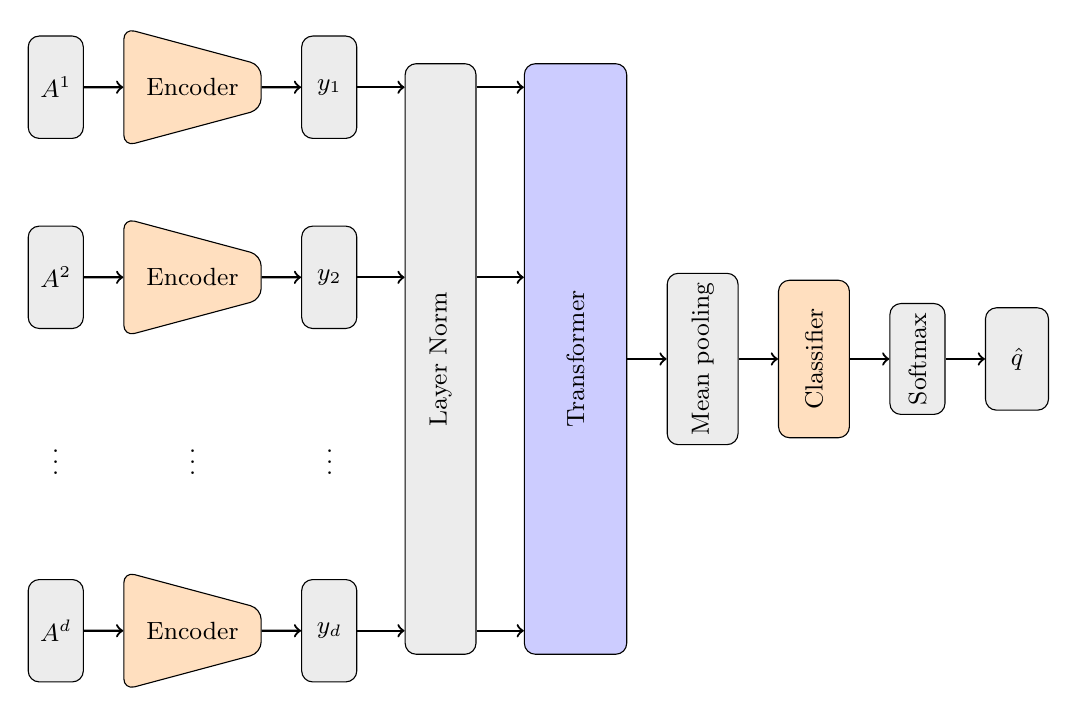
\begin{tikzpicture}[ 
        % node distance: vertical=1.1cm, horizontal=0.5cm (reduced from 0.9cm)
        node distance=1.1cm and 0.5cm,
        every node/.style={font=\small},
        data/.style={draw, rounded corners, fill=gray!15,
                     minimum width=0.7cm, minimum height=1.3cm},
        pool/.style={draw, rounded corners, fill=gray!15,
                     minimum width=0.9cm, minimum height=1.4cm},
        norm/.style={draw, rounded corners, fill=gray!15,
                     minimum width=0.9cm, minimum height=7.5cm},
        classifier/.style={draw, rounded corners, fill=orange!25,
                           minimum width=0.9cm, minimum height=2.0cm},
        transformer/.style={draw, rounded corners, fill=blue!20,
                            minimum width=1.3cm, minimum height=7.5cm}, 
        arrow/.style={->, thick},
        encoder/.style={
            draw, trapezium, trapezium angle=75,
            shape border rotate=270,
            fill=orange!25,
            rounded corners,
            minimum width=1.5cm,
            minimum height=0.9cm
        }
    ]
    
    % --- Inputs ---
    \node[data] (A1) {$A^1$};
    \node[data, below=of A1] (A2) {$A^2$};
    \node[below=1.2cm of A2] (dots_input) {\vdots}; 
    \node[data, below=1.2cm of dots_input] (Ar) {$A^d$};
    
    % --- Encoders ---
    \node[encoder, right=of A1] (E1) {Encoder};
    \node[encoder, right=of A2] (E2) {Encoder};
    \node[right=1.4cm of dots_input] (dots_enc) {\vdots}; 
    \node[encoder, right=of Ar] (Er) {Encoder};
    
    % --- y outputs ---
    \node[data, right=of E1] (y1) {$y_1$};
    \node[data, right=of E2] (y2) {$y_2$};
    \node[right=1.4cm of dots_enc] (dots_y) {\vdots}; 
    \node[data, right=of Er] (yr) {$y_d$};
    
    % --- Right Side (Vertically Centered) ---
    \coordinate (centerpoint) at ($(y1.east)!0.5!(yr.east)$);
    
    % Layer Norm placed between y outputs and Transformer
    \node[norm, right=0.6cm of centerpoint] (LN) {\rotatebox{90}{Layer Norm}};
    \node[transformer, right=0.6cm of LN] (T) {\rotatebox{90}{Transformer}};
    \node[pool, right=of T] (MP) {\rotatebox{90}{Mean pooling}};
    \node[classifier, right=of MP] (C) {\rotatebox{90}{Classifier}};
    \node[data, right=of C] (L) {\rotatebox{90}{Softmax}};
    \node[data, right=of L, minimum width=0.8cm] (Q) {\rotatebox{0}{$\hat{q}$}};
    
    % --- Arrows ---
    \draw[arrow] (A1) -- (E1);
    \draw[arrow] (A2) -- (E2);
    \draw[arrow] (Ar) -- (Er);
    
    \draw[arrow] (E1) -- (y1);
    \draw[arrow] (E2) -- (y2);
    \draw[arrow] (Er) -- (yr);
    
    % Symmetrical arrows into Layer Norm
    \draw[arrow] (y1.east) -- (LN.west |- y1.east);
    \draw[arrow] (y2.east) -- (LN.west |- y2.east);
    \draw[arrow] (yr.east) -- (LN.west |- yr.east);
    
    % Connection from Layer Norm to Transformer
    \draw[arrow] (LN.east |- y1.east) -- (T.west |- y1.east);
    \draw[arrow] (LN.east |- y2.east) -- (T.west |- y2.east);
    \draw[arrow] (LN.east |- yr.east) -- (T.west |- yr.east);
    
    % Right side flow
    \draw[arrow] (T) -- (MP);
    \draw[arrow] (MP) -- (C);
    \draw[arrow] (C) -- (L);
    \draw[arrow] (L) -- (Q);
    
\end{tikzpicture}
\end{document}